\chapter{Results}
\label{chapter:results}

In this chapter, I evaluate the performance of my architecture on the GQA dataset using a combination of traditional accuracy measures and GQA-specific metrics. First, I compare my architecture to the collection of baseline VQA methods introduced in the previous chapter. Secondly, I present results for variations of my model, replacing or entirely removing its question and/or scene graph processing modules to justify my architecture design. Finally, I delve into the parameter configuration of my model, exploring how parameters such as learning rate, reasoning module length and scene graph module size affect the performance of my model and the methods I used to find my final parameter configuration.

\section{Performance Evaluation}
\label{section:performance_evaluation}

\begin{table}[htbp]
    \begin{footnotesize}
        \begin{tabularx}{\linewidth}{L|c|cc|ccc}
            \toprule
            \multirow{2}{*}{\textbf{Model}} & \multicolumn{6}{c}{\textbf{GQA}} \\
            \cmidrule{2-7}
            & Accuracy & Binary & Open & Validity & Plausibility & Distribution \\
            \midrule
            Human \cite{hudson2019gqa} & 89.30 & 91.20 & 87.40 & 98.90 & 97.20 & - \\
            \midrule
            LXMERT \cite{tan2019lxmert, tan2019lxmertgithub}& 59.80 & - & - & - & - & - \\
            BAN-4 \cite{kim2018bilinear, guo2019bilinear} & 61.95 & - & - & - & - & - \\
            GRN \cite{guo2019bilinear} & 64.22 & - & - & - & - & - \\
            % MCAN \cite{yu2019deep, farazi2020attention} & 65.00 & 82.08 & 48.98 & 94.91 & 91.42 & 4.21\\
            MSA\cite{farazi2020attention} & 65.93 & 82.35 & 49.27 & 94.98 & 91.57 & 4.88\\
            \midrule
            MSA\(^{\dag}\) \cite{farazi2020attention} & 68.71 & 71.84 & 68.71 & 94.94 & 92.99 & 7.29\\
            MAC\(^\dag\) \cite{hudson2018compositional} & 73.64 & 81.86 & 65.94 & \textbf{95.38} & 92.46 & 2.05 \\
            MSA\(^{\ddag}\) \cite{farazi2020attention} & 81.15 & 85.06 & 77.48 & \textbf{95.34} & 94.26 & 1.08\\
            \midrule
            \textbf{Our Model}\(^\dag\) & \textbf{90.30} & \textbf{91.59} & \textbf{89.10} & \textbf{95.35} & \textbf{94.48} & \textbf{0.29} \\
            \bottomrule
        \end{tabularx}
        \caption[A performance comparison of various models on the GQA validation set.]{A comparison of the performance of various models on the GQA validation set. Human performance is based on majority vote of 5 human responses for 4000 random GQA questions. Models marked with a \(^\dag\) have access to pre-annotated GQA scene graph objects, attributes and relations at inference time, and models marked with a \(^\ddag\) use Faster R-CNN \cite{ren2016faster} features and/or bounding box information in addition to scene graph information. Where two citations are provided, the first corresponds to the original paper and the second corresponds to the source of the validation set results.}
        \label{table:performance_comparison}
    \end{footnotesize}
\end{table}

As demonstrated in \tableautorefname{ \ref{table:performance_comparison}}, my model outperforms all baseline models by a significant margin across all accuracy metrics, and performs on par or slightly better than reported models for GQA validity, plausibility and distribution. Moreover, it outperforms human baseline performance for all accuracy measures.

For fairness of comparison, I split baseline model performance into two sections; all models in the upper section use only Faster R-CNN and/or bounding box information during evaluation time, where all models in the lower section have access to GQA scene graph object, attribute and relationship data.

Stepping through each of the baselines in the upper section of \tableautorefname{ \ref{table:performance_comparison}}, it becomes evident how important the type of visual signal is for VQA models; we see that my model outperforms all four baselines that only have access to object and bounding box features by anywhere from 30.5\% in the case of LXMERT \cite{tang2019learning} to 24.37\% in the case of MSA \cite{farazi2020attention} when comparing overall accuracy. Since I use pre-annotated scene graphs from the GQA dataset as my model's visual signal, it makes sense that my model outperforms existing baselines that don't have access to this information. Moreover, we see that whilst my model outperforms MSA by 24.37\% in overall accuracy, the difference between the two models closes to only 9.24\% for binary-type questions, but grows to almost 50\% for open-type questions. Moreover, we see that my model has a much lower distribution than MSA, meaning it relies less on statistical priors in the dataset when forming its answers, and more on its visual input. Again, this is easily explained by the advantage of pre-annotated scene graph information. Interestingly, the difference in performance between my model and MSA on the validity and plausibility metrics is much less pronounced, at only 0.37\% and 2.91\% respectively. This is due to two primary reasons:

\begin{itemize}
    \item Validity and plausibility are much more forgiving metrics than accuracy. Validity is the most forgiving, since a model only has to provide an answer of the correct type \textit{e.g. provide a colour when the question about the colour of an object}. Plausibility is less forgiving than validity but still more forgiving than accuracy, since the provided answer has to make sense given the context of the question and image. As a result, the difference between validity for the two models is the smallest, followed by plausibility and then finally accuracy.
    \item Providing a valid or plausible answer does not always require visual information. We see this phenomenon in the results on the GQA test set in the original GQA publication \cite{hudson2019gqa}, where a language only LSTM model provides valid answers between 0.37\% and 0.21\% more often than the CNN + LSTM, BottomUp \cite{anderson2018bottom} and MAC \cite{hudson2018compositional} baselines, and provides plausible answers between 2.73\% and 3.05\% more often. Consequently, despite having a much weaker visual signal than my model, the MSA model in the upper section of \tableautorefname{ \ref{table:performance_comparison}} still performs comparably on the validity and plausibility metrics.
\end{itemize}

These observations extend to models in the lower section of \tableautorefname{ \ref{table:performance_comparison}}, which perform almost identically to my model on the validity metric, and between 0.2-2.0\% worse than my model for answer plausibility.

Moving our focus to the lower section of \tableautorefname{ \ref{table:performance_comparison}}, we see that the baseline models perform much better than those in the upper section, as they also have GQA scene graph information at their disposal. Importantly, we see that my model is still over 9.1\% more accurate than MSA despite not using any Faster R-CNN object features. When we remove Faster R-CNN features from MSA, we see a drop of almost 13\%, making my model almost 22.6\% more accurate than MSA given the same underlying information. Moreover, a MAC network that uses the same question encoding method as my model and uses GloVe embeddings for scene graph object, attributes and relations is still outperformed by my model by almost 16.7\%, highlighting the importance of the scene graph embedding and processing module in my final model.

Examining accuracy for binary and open question types, we see that while all three models that use scene graph information have a significantly lower (between 3.1-7.5\%) open-type accuracy compared to their binary-type accuracy, my model answers binary and open questions almost equally well, with only a 2.49\% difference between the two.

% TODO save for MSA
% Even though LXMERT \cite{tang2019learning} utilises the renowned transformer encoder \cite{vaswani2017attention} to embed visual Faster R-CNN and bounding box region features, it still has the arduous task of reconciling visual information with information from the question. Transformers have proven to be extremely capable in the Natural Language Processing (NLP) field, as their attention mechanisms operate well when their inputs are drawn from the same semantic space. Unfortunately, it is still not well-known how well scaled dot-product attention mechanisms like those found in transformers perform in multi-modal contexts, meaning the cross-modal transformer architecture used by LXMERT may have a hard time reconciling textual and visual features. Conversely, my model embeds both textual and visual information using GloVe vectors \cite{pennington2014glove}, meaning that both question and scene graph features are similar in their distributions and can consequently be compared easily using attention mechanisms. Consequently, my model performs an incredible 30.50\% better than LXMERT, however I posit that if LXMERT was to use similar embeddings for both textual and visual data, this gap would close significantly.

Based on the results in \tableautorefname{ \ref{table:performance_comparison}}, I believe the primary contributor to my model's excellent performance is its scene graph embedding and processing method. All three models in the lower half of the table use semantic word embeddings to represent scene graph objects, relations and attributes, and use attention-based reasoning methods. Consequently, the main point of differentiation between my model and the others is the use of graph attention networks (GATs) to process scene graph information. I confirm this hypothesis in \subsectionautorefname{ \ref{subsec:scene_graph_module_ablations}}, where I implement multiple scene graph processing module alternatives and demonstrate the effectiveness of GATs for learning semantically-rich scene graph embeddings.

\section{Ablation Studies}
\label{sec:ablation_studies}

To gain a more complete understanding of how the components of my model contribute to its performance, I explore how removing or replacing certain parts of my model change its behaviour. More specifically, I report how changes to the question processing module and scene graph processing module affect the performance of my model, investigating performance at a macro level using the metrics seen in the previous section, as well as at a micro level, examining model accuracy as a function of question length, question complexity and question structural and semantic types.  

For all ablation studies in this chapter, I train models on the balanced GQA training set and split the balanced GQA validation set in half, reserving the first half for parameter optimisation and the second half for testing. Consequently, all results reported in this section are computed on the second half of the balanced GQA validation set, instead of the full validation set like in \tableautorefname{ \ref{table:performance_comparison}}, to avoid giving an unfair advantage to my best model, which was tuned using the first half of the balanced validation set.

Before delving into ablation study results, it is important to understand the underlying distributions of the test set used to compute various metrics. As illustrated in \figureautorefname{ \ref{fig:test_structural_and_semantic_distribution}}, the second half of the GQA validation set has a very similar semantic and structural type distribution to the rest of the balanced GQA dataset. Examining the semantic type distribution, we see that 46.6\% of questions query about the relationships between objects, 31.8\% ask about attributes, 11.8\% about objects, 6.6\% about object categories and 3.1\% about global properties. Regarding structural types, 51.7\% of questions are open-type questions that query about scene properties in general, 20.7\% of questions require verifying some property about the scene, 12.3\% require logical reasoning operations, 12.2\% require choosing between a set of options provided in the question and 3.1\% require comparing the properties of two or more objects. 

\begin{figure}[htbp]
    \centering
    \begin{subfigure}[l]{0.4\textwidth}
        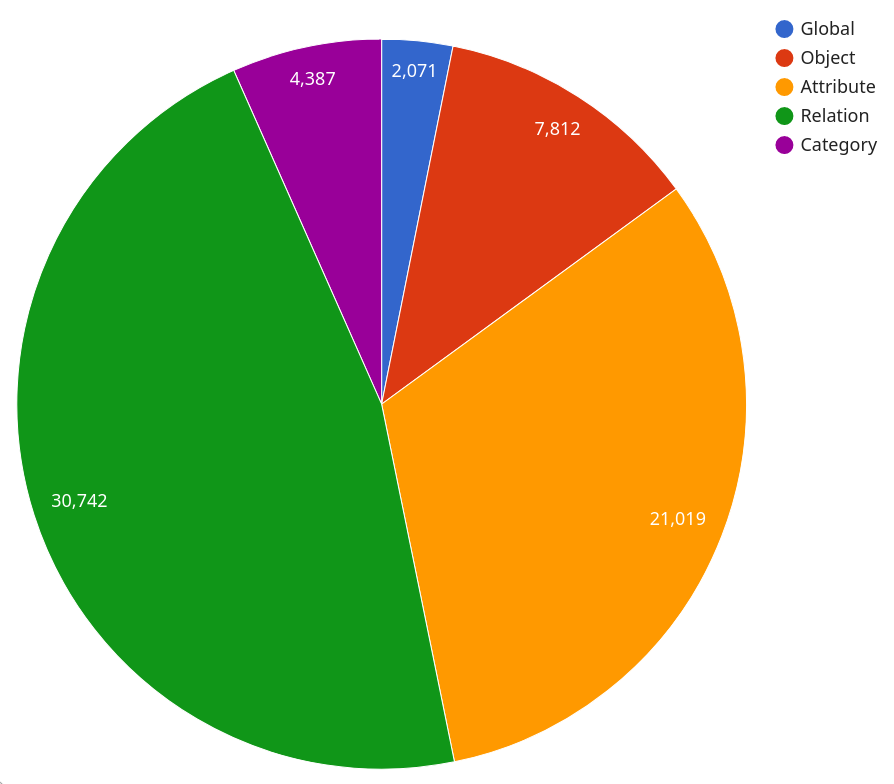
\includegraphics[width=\textwidth]{gqa_semantic_types.png}
        \label{fig:test_semantic_types}
        \caption{GQA semantic type distribution.}
    \end{subfigure}
    \begin{subfigure}[r]{0.4\textwidth}
        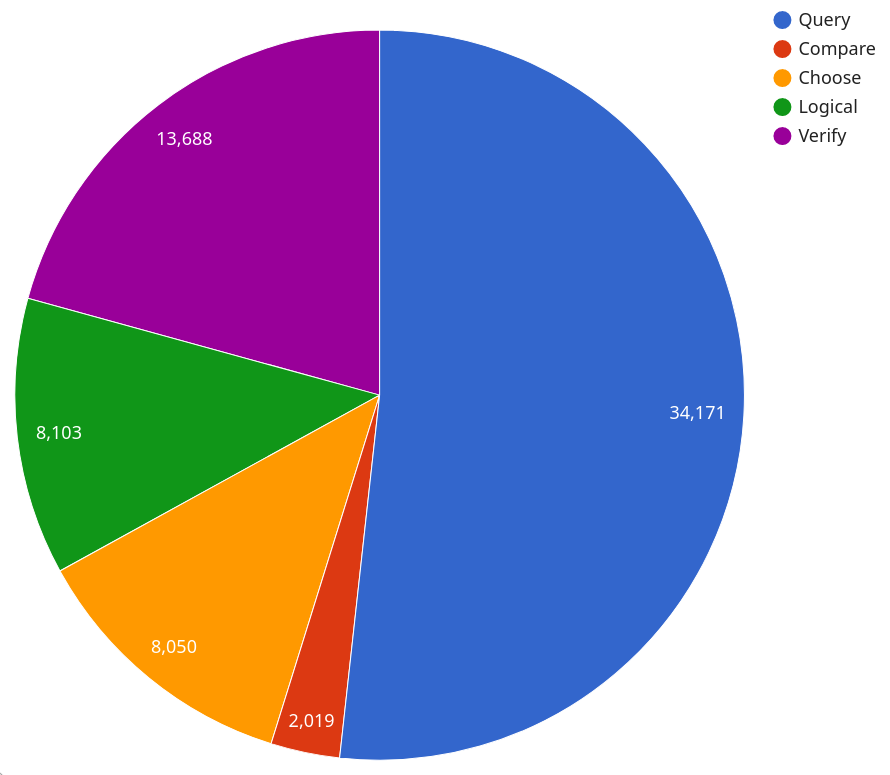
\includegraphics[width=\textwidth]{gqa_structural_types.png}
        \label{fig:test_structural_types}
        \caption{GQA structural type distribution.}
    \end{subfigure}
    \caption[GQA structural and semantic question type distributions.]{Distribution of structural and semantic question types across the second half of the balanced GQA validation set.}
    \label{fig:test_structural_and_semantic_distribution}
\end{figure}

\figureautorefname{ \ref{fig:test_reasoning_step_and_question_length_distribution}} illustrates the compositional nature of the questions in the GQA dataset, with the majority of questions requiring 2-3 discrete reasoning steps to arrive at an answer. We also see that most questions contain around 5 to 11 words, however there are still a large number of longer questions that a good VQA model needs to be able to interpret.

\begin{figure}[htbp]
    \centering
    \begin{subfigure}[l]{0.5\textwidth}
        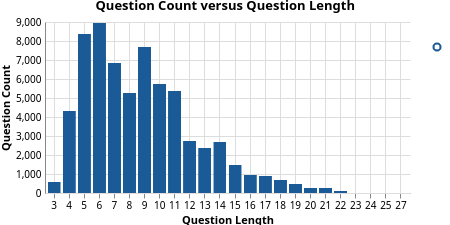
\includegraphics[width=\textwidth]{test_question_count_vs_question_length.png}
        \label{fig:test_question_length_distribution}
    \end{subfigure}
    \begin{subfigure}[r]{0.49\textwidth}
        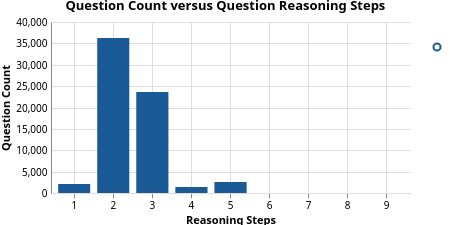
\includegraphics[width=\textwidth]{test_question_count_vs_reasoning_steps.png}
        \label{fig:test_reasoning_step_distribution}
    \end{subfigure}
    \caption[GQA question length and reasoning step count distributions.]{Distribution of questions across the second half of the balanced GQA validation set for both question length and reasoning step count.}
    \label{fig:test_reasoning_step_and_question_length_distribution}
\end{figure}



\subsection{Question Module Ablations}
\label{subsec:question_module_ablations}

In this \subsectionautorefname, I explore three alternative question processing modules, namely a convolutional neural network (CNN) inspired by work on sentence classification in the NLP field \cite{kim2014convolutional}, a graph convolutional network (GCN) that uses synactic dependencies as edges, and a graph attention network (GAT) that operates in a similar fashion to the GCN but learn individual weights for each syntactic dependency. Moreover, I investigate the effects of removing the question processing module entirely, relying purely on GloVe embeddings as a question input signal. Before delving into results, I provide a brief overview of how each of these ablations fit in to the rest of my model architecture, adopting notation from \chapterautorefname{ \ref{chapter:methodology}}.

\textbf{CNN}: Modeled on the architecture presented in \cite{kim2014convolutional}, the CNN question processing module takes a batch of raw question embeddings \(H_{Q_{[i:i+k]}} \in \R^{k \times l \times d_{H_q}}\) as its input and applies multiple 2D convolutions of varying receptive fields in parallel to learn a contextual representation of each question. I use a total of four Conv2D layers, each with 128 output channels and kernel sizes of \((3 \times d_{H_q})\), \((5 \times d_{H_q})\), \((7 \times d_{H_q})\) and \((9 \times d_{H_q})\). Appropriate padding is applied for each Conv2D layer so that convolved features for each layer are always of size \(l \times 128\). The convolved features for each layer are concatenated together to yield \(K_{Q_{[i:i+k]}} \in \R^{k \times l \times 512}\), the knowledge-base of contextual words used as an input to the reasoning module. After obtaining convolved features for each question in the batch, I take the maximum value of each output channel across the question length dimension to obtain a single vector \(\mathcal{Q}_q\) of dimension 512, representing the question as a whole. When processed as a batch, this yields a matrix of question representations \(\mathcal{Q}_{Q_{[i:i+k]} } \in \R^{k \times 512}\).

\textbf{GCN \& GAT}: As mentioned in the footnotes in \sectionautorefname{ \ref{section:question_embedding_and_module}}, during the question preprocessing stage I retrieve syntactic dependencies for each question using the Stanza NLP package \cite{qi2020stanza}. These syntactic dependencies form the edges of a question graph, and the node embeddings \(H_{Q_{[i:i+k]}} \in \R^{k \times l \times d_{H_q}}\) are obtained in a similar manner to the scene graph node embedding creation process as described in \subsectionautorefname{ \ref{sec:scene_graph_embedding_details}}. This yields a question graph \(\mathcal{G}_q = (\mathcal{V}_q, \mathcal{E}_q)\), where \(|\mathcal{V}_q| = l_q\) and \(|\mathcal{E}_q| = l_q - 1\).


\begin{table}[htbp]
\centering
\begin{footnotesize}
\begin{tabularx}{\linewidth}{CC|c|cc|ccc}
\toprule
\multirow{3}{0.1\textwidth}{\textbf{Question Module}} & \multirow{3}{0.1\textwidth}{\textbf{Scene Graph Module}} & \multicolumn{6}{c}{\multirow{2}{*}{\textbf{GQA}}}                                                                                                                                         \\
                                          &                                              & \multicolumn{6}{c}{}                                                                                                                                                                      \\ \cmidrule(l){3-8} 
                                          &                                              & \multicolumn{1}{l}{Accuracy} & \multicolumn{1}{l}{Binary} & \multicolumn{1}{l}{Open} & \multicolumn{1}{l}{Validity} & \multicolumn{1}{l}{Plausibility} & \multicolumn{1}{l}{Distribution} \\ \midrule
None                                      & GAT                                          & 86.52                        & 85.78                      & 87.21                    & 95.10                         & 93.85                            & 0.26                             \\
CNN                                       & GAT                                          & 87.35                        & 87.87                      & 86.86                    & 95.24                        & 94.22                            & 0.29                             \\
GAT                                       & GAT                                          & 89.43                        & \textbf{91.88}             & 87.16                    & 95.26                        & 94.19                            & 0.27                             \\
GCN                                       & GAT                                          & 86.02                        & 86.77                      & 85.32                    & 95.05                        & 93.92                            & 0.34                             \\
BiLSTM                                    & GAT                                          & \textbf{90.45}               & 91.73                      & \textbf{89.26}           & \textbf{95.34}                        & \textbf{94.48}                   & \textbf{0.19}                    \\
\bottomrule
\end{tabularx}
\end{footnotesize}
\end{table}



\begin{table}[htbp]
\centering
\begin{footnotesize}
\begin{tabular}{cc|c|ccccc}
\toprule
\multirow{3}{0.1\textwidth}{\textbf{Question Module}} & \multirow{3}{0.1\textwidth}{\textbf{Scene Graph Module}} & \multicolumn{6}{c}{\multirow{2}{*}{\textbf{GQA}}}                                                   \\
                                          &                                              & \multicolumn{6}{c}{}                                                                                \\ \cmidrule(l){3-8} 
                                          &                                              & Accuracy       & Query          & Compare        & Choose         & Logical        & Verify         \\ \midrule
None                                      & GAT                                          & 86.52          & 87.21          & 80.44          & 78.89          & 93.77          & 85.88          \\
CNN                                       & GAT                                          & 87.35          & 86.86          & 67.66          & 85.99          & 92.57          & 89.17          \\
GAT                                       & GAT                                          & 89.43          & 87.16          & \textbf{93.02} & 86.92          & 96.43          & 91.93          \\
GCN                                       & GAT                                          & 86.02          & 85.32          & 73.60          & 84.96          & 92.85          & 86.17          \\
BiLSTM                                    & GAT                                          & \textbf{90.45} & \textbf{89.26} & 69.69          & \textbf{90.87} & \textbf{97.45} & \textbf{92.10} \\ \bottomrule
\end{tabular}
\end{footnotesize}
\end{table}

{\color{red}Things to note: High compare score whenever we use the same question and scene graph module! e.g. GAT and GAT in this case}


\begin{table}[htbp]
\centering
\begin{footnotesize}
\begin{tabular}{cc|c|ccccc}
\toprule
\multirow{3}{0.1\textwidth}{\textbf{Question Module}} & \multirow{3}{0.1\textwidth}{\textbf{Scene Graph Module}} & \multicolumn{6}{c}{\multirow{2}{*}{\textbf{GQA}}}                                                   \\
                                          &                                              & \multicolumn{6}{c}{}                                                                                \\ \cmidrule(l){3-8} 
                                          &                                              & Accuracy       & Global         & Object         & Attribute      & Relation       & Category       \\ \midrule
None                                      & GAT                                          & 86.52          & \textbf{83.97}          & 94.75          & 87.35          & 83.67          & 89.01          \\
CNN                                       & GAT                                          & 87.35          & 83.78          & 93.63          & 85.37          & 87.37          & 87.14          \\
GAT                                       & GAT                                          & 89.43          & 83.82          & 97.24          & \textbf{89.74} & 87.88          & 87.62          \\
GCN                                       & GAT                                          & 86.02          & 83.39          & 93.36          & 83.65          & 86.32          & 83.43          \\
BiLSTM                                    & GAT                                          & \textbf{90.45} & 83.92          & \textbf{97.39} & 88.39          & \textbf{90.51} & \textbf{90.65} \\ \bottomrule
\end{tabular}
\end{footnotesize}
\end{table}

\begin{figure}[htbp]
    \centering
    \begin{subfigure}[l]{0.5\textwidth}
        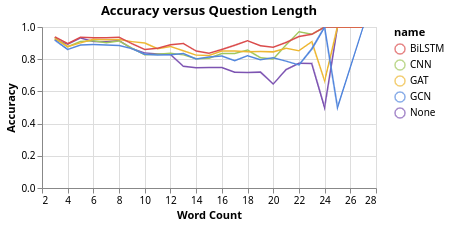
\includegraphics[width=\textwidth]{accuracy_vs_question_length_question_ablation.png}
        \label{fig:accuracy_vs_question_length_question_ablation}
    \end{subfigure}
    \begin{subfigure}[r]{0.49\textwidth}
        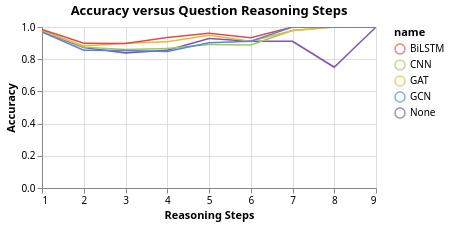
\includegraphics[width=\textwidth]{accuracy_vs_reasoning_steps_question_ablation.png}
        \label{fig:accuracy_vs_reasoning_steps_question_ablation}
    \end{subfigure}
    \caption{Per-question-length and per-reasoning-step accuracy for various question processing module types.}
\end{figure}

The high performance of the right-hand tails in both cases are due to the small number of questions with a large number of words or reasoning steps, as illustrated in \figureautorefname{ \ref{fig:test_reasoning_step_and_question_length_distribution}}

\subsection{Scene Graph Module Ablations}
\label{subsec:scene_graph_module_ablations}

\begin{table}[htbp]
\centering
\begin{footnotesize}
\begin{tabularx}{\linewidth}{CC|c|cc|ccc}
\toprule
\multirow{3}{0.1\textwidth}{\textbf{Question Module}} & \multirow{3}{0.1\textwidth}{\textbf{Scene Graph Module}} & \multicolumn{6}{c}{\multirow{2}{*}{\textbf{GQA}}}                                                                                                                                         \\
                                          &                                              & \multicolumn{6}{c}{}                                                                                                                                                                      \\ \cmidrule(l){3-8} 
                                          &                                              & \multicolumn{1}{l}{Accuracy} & \multicolumn{1}{l}{Binary} & \multicolumn{1}{l}{Open} & \multicolumn{1}{l}{Validity} & \multicolumn{1}{l}{Plausibility} & \multicolumn{1}{l}{Distribution} \\ \midrule
BiLSTM                                    & None                                         & 73.63                        & 81.84                      & 65.98                    & \textbf{95.38}               & 92.46                            & 1.09                    \\
BiLSTM                                    & BiLSTM                                       & 83.35                        & 85.81                      & 81.06                    & 95.27                        & 93.73                            & 0.31                             \\
BiLSTM                                    & GCN                                          & 69.44                        & 78.14                      & 61.34                    & 95.13                        & 91.95                            & 1.11                             \\
BiLSTM                                    & GAT                                          & \textbf{90.45}               & \textbf{91.73}                      & \textbf{89.26}           & 95.34                        & \textbf{94.48}                   & \textbf{0.19}                    \\
\bottomrule
\end{tabularx}
\end{footnotesize}
\end{table}

\begin{table}[htbp]
\centering
\begin{footnotesize}
\begin{tabular}{cc|c|ccccc}
\toprule
\multirow{3}{0.1\textwidth}{\textbf{Question Module}} & \multirow{3}{0.1\textwidth}{\textbf{Scene Graph Module}} & \multicolumn{6}{c}{\multirow{2}{*}{\textbf{GQA}}}                                                   \\
                                          &                                              & \multicolumn{6}{c}{}                                                                                \\ \cmidrule(l){3-8} 
                                          &                                              & Accuracy       & Query          & Compare        & Choose         & Logical        & Verify         \\ \midrule
BiLSTM                                    & None                                         & 73.63          & 65.98          & 69.44          & 72.84          & 92.85          & 82.44          \\
BiLSTM                                    & BiLSTM                                       & 83.35          & 81.06          & \textbf{92.22}          & 73.98          & 95.79          & 85.91          \\
BiLSTM                                    & GCN                                          & 69.44          & 61.34          & 66.37          & 71.04          & 85.96          & 79.43          \\
BiLSTM                                    & GAT                                          & \textbf{90.45} & \textbf{89.26} & 69.69          & \textbf{90.87} & \textbf{97.45} & \textbf{92.10} \\ \bottomrule
\end{tabular}
\end{footnotesize}
\end{table}

\begin{table}[htbp]
\centering
\begin{footnotesize}
\begin{tabular}{cc|c|ccccc}
\toprule
\multirow{3}{0.1\textwidth}{\textbf{Question Module}} & \multirow{3}{0.1\textwidth}{\textbf{Scene Graph Module}} & \multicolumn{6}{c}{\multirow{2}{*}{\textbf{GQA}}}                                                   \\
                                          &                                              & \multicolumn{6}{c}{}                                                                                \\ \cmidrule(l){3-8} 
                                          &                                              & Accuracy       & Global         & Object         & Attribute      & Relation       & Category       \\ \midrule
BiLSTM                                    & None                                         & 73.63          & \textbf{85.18} & 95.15          & 64.46          & 72.38          & 82.54          \\
BiLSTM                                    & BiLSTM                                       & 83.35          & 82.86          & 95.60          & 80.88          & 81.02          & 89.92          \\
BiLSTM                                    & GAT                                          & \textbf{90.45} & 83.92          & \textbf{97.39} & \textbf{88.39}          & \textbf{90.51} & \textbf{90.65} \\
BiLSTM                                    & GCN                                          & 69.44          & 70.45          & 87.54          & 67.22          & 66.25          & 69.77          \\
\bottomrule
\end{tabular}
\end{footnotesize}
\end{table}


\begin{figure}[htbp]
    \centering
    \begin{subfigure}[l]{0.5\textwidth}
        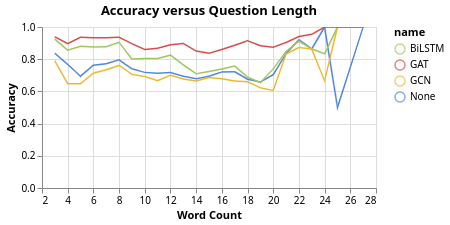
\includegraphics[width=\textwidth]{accuracy_vs_question_length_scene_graph_ablation.png}
        \label{fig:accuracy_vs_question_length_scene_graph_ablation}
    \end{subfigure}
    \begin{subfigure}[r]{0.49\textwidth}
        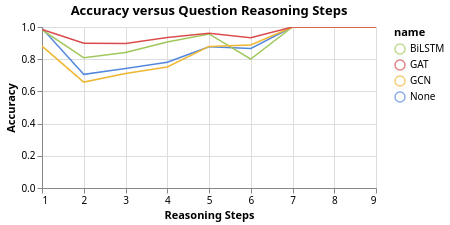
\includegraphics[width=\textwidth]{accuracy_vs_reasoning_steps_scene_graph_ablation.png}
        \label{fig:accuracy_vs_reasoning_steps_scene_graph_ablation}
    \end{subfigure}
    \caption{Per-question-length and per-reasoning-step accuracy for various scene graph processing module types.}
\end{figure}

The high performance of the right-hand tails in both cases are due to the small number of questions with a large number of words or reasoning steps, as illustrated in \figureautorefname{ \ref{fig:test_reasoning_step_and_question_length_distribution}}


{\color{red}Things to note: High compare score whenever we use the same question and scene graph module! e.g. BiLSTM and BiLSTM in this case}

{\color{red}TODO: GloVe only for scene graph and questions}

{\color{red}TODO: Ablations on scene graph embedding for best model only:
\begin{itemize}
    \item Removal of skip-edges in the graph
    \item Removal of relation data, with edges only occurring between objects where a relation would usually be (i.e. skip edges w/ no relation nodes)
    \item If time, removal of relation and attribute data as well.
\end{itemize}}

\begin{itemize}
    \item Includes more important initial tests, move less important ones to appendix.
\end{itemize}

\begin{itemize}
    \item GloVe vs random normal distribution. Glove required less tuning since the vector norms already worked well.
\end{itemize}

\section{Hyperparameter Optimisation}
\label{sec:hyperparameter_optimisation}

Rigorous initial tests were performed - reported and non-reported results represent 159 days of GPU computation time.

These results represent a total of 55 days of GPU compute

{\color{red}
  \begin{itemize}
    \item \textit{Weights \& Biases} \cite{wandb} implementation of bayesian optimisation, using the hyperband early stopping method
    \item Include results using LeakyReLU between GAT layers?
  \end{itemize}
}



The effects of the Hyperband method are clearly seen in \figureautorefname{ \ref{fig:hyperparameter_optimisation_validation_loss_and_accuracy}}, where only a few models are trained to completion and less promising models are stopped earlier to encourage exploration of the hyperparameter search space.

\begin{figure}
    \centering
    \begin{subfigure}[t]{\textwidth}
        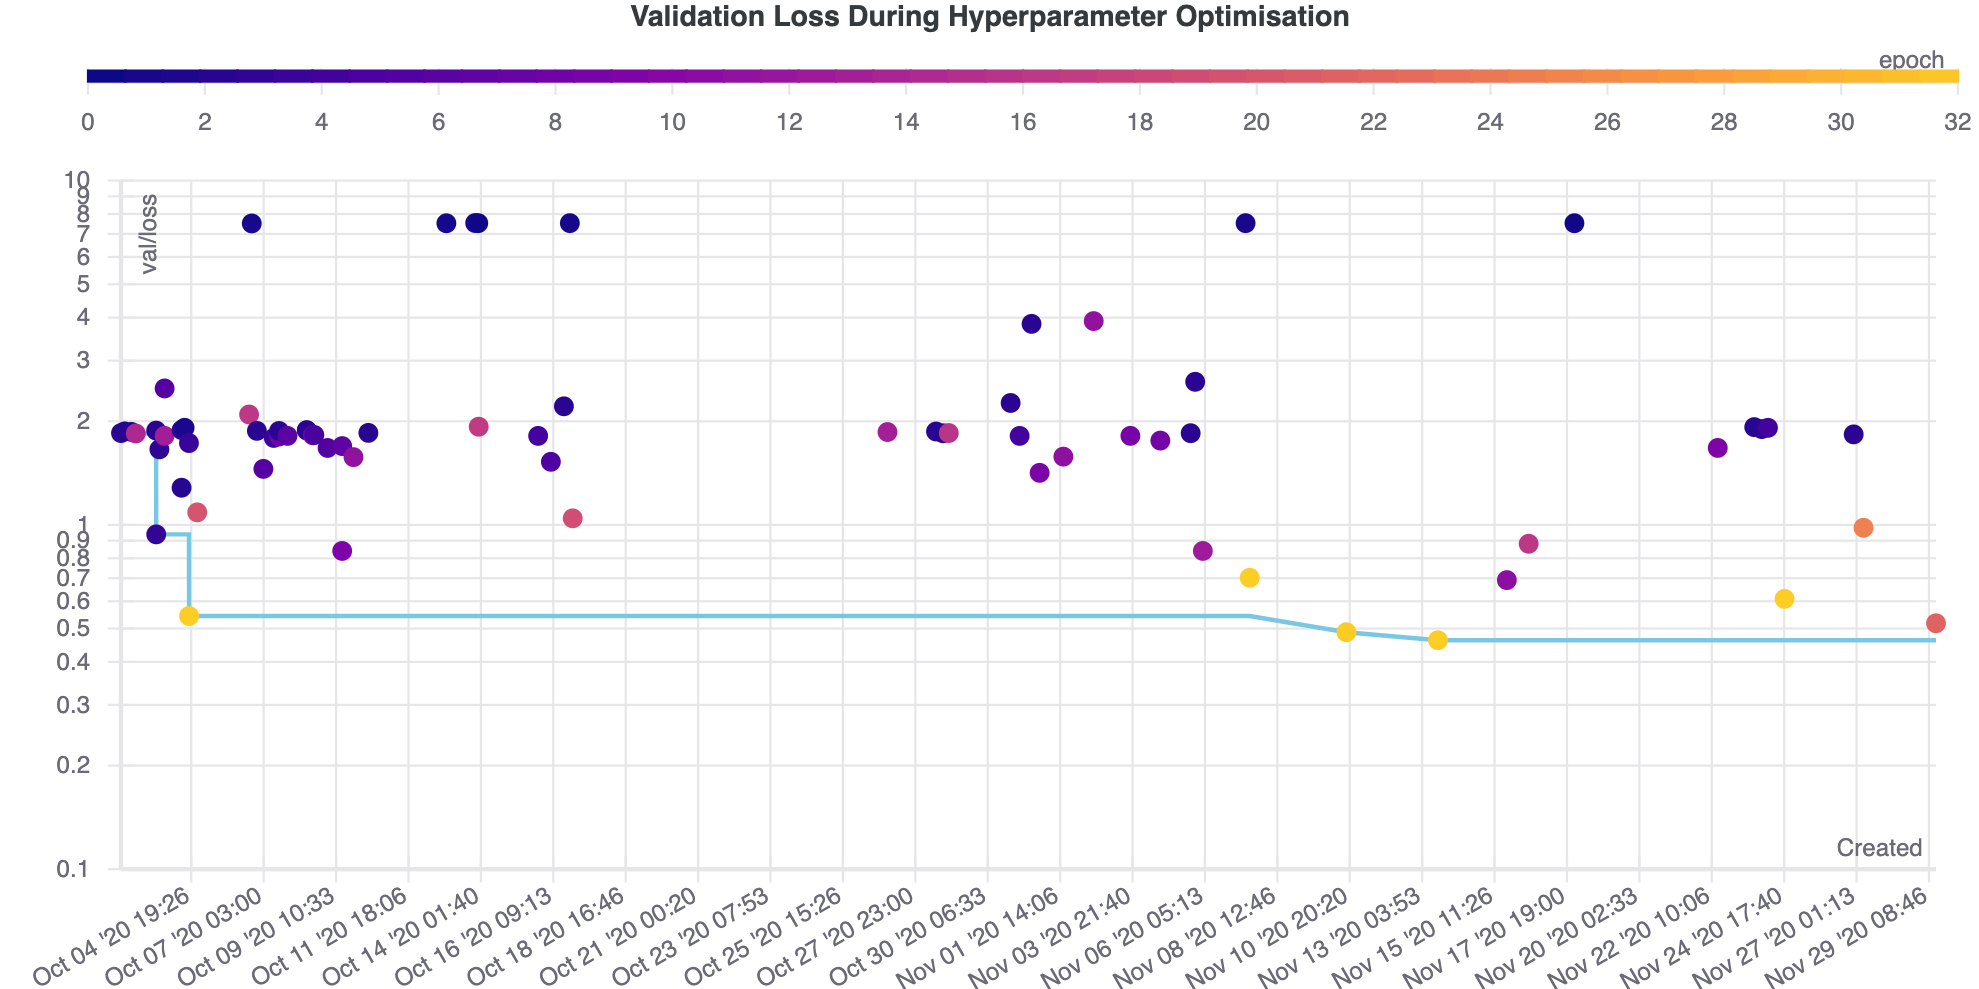
\includegraphics[width=\textwidth]{hyperparameter_optimisation_validation_loss.png}
        \label{fig:hyperparameter_optimisation_validation_loss}
        \caption{Validation loss throughout the hyperparameter optimisation process.}
    \end{subfigure}
    \par\bigskip % force a bit of vertical whitespace
    \par\bigskip
    \begin{subfigure}[b]{\textwidth}
        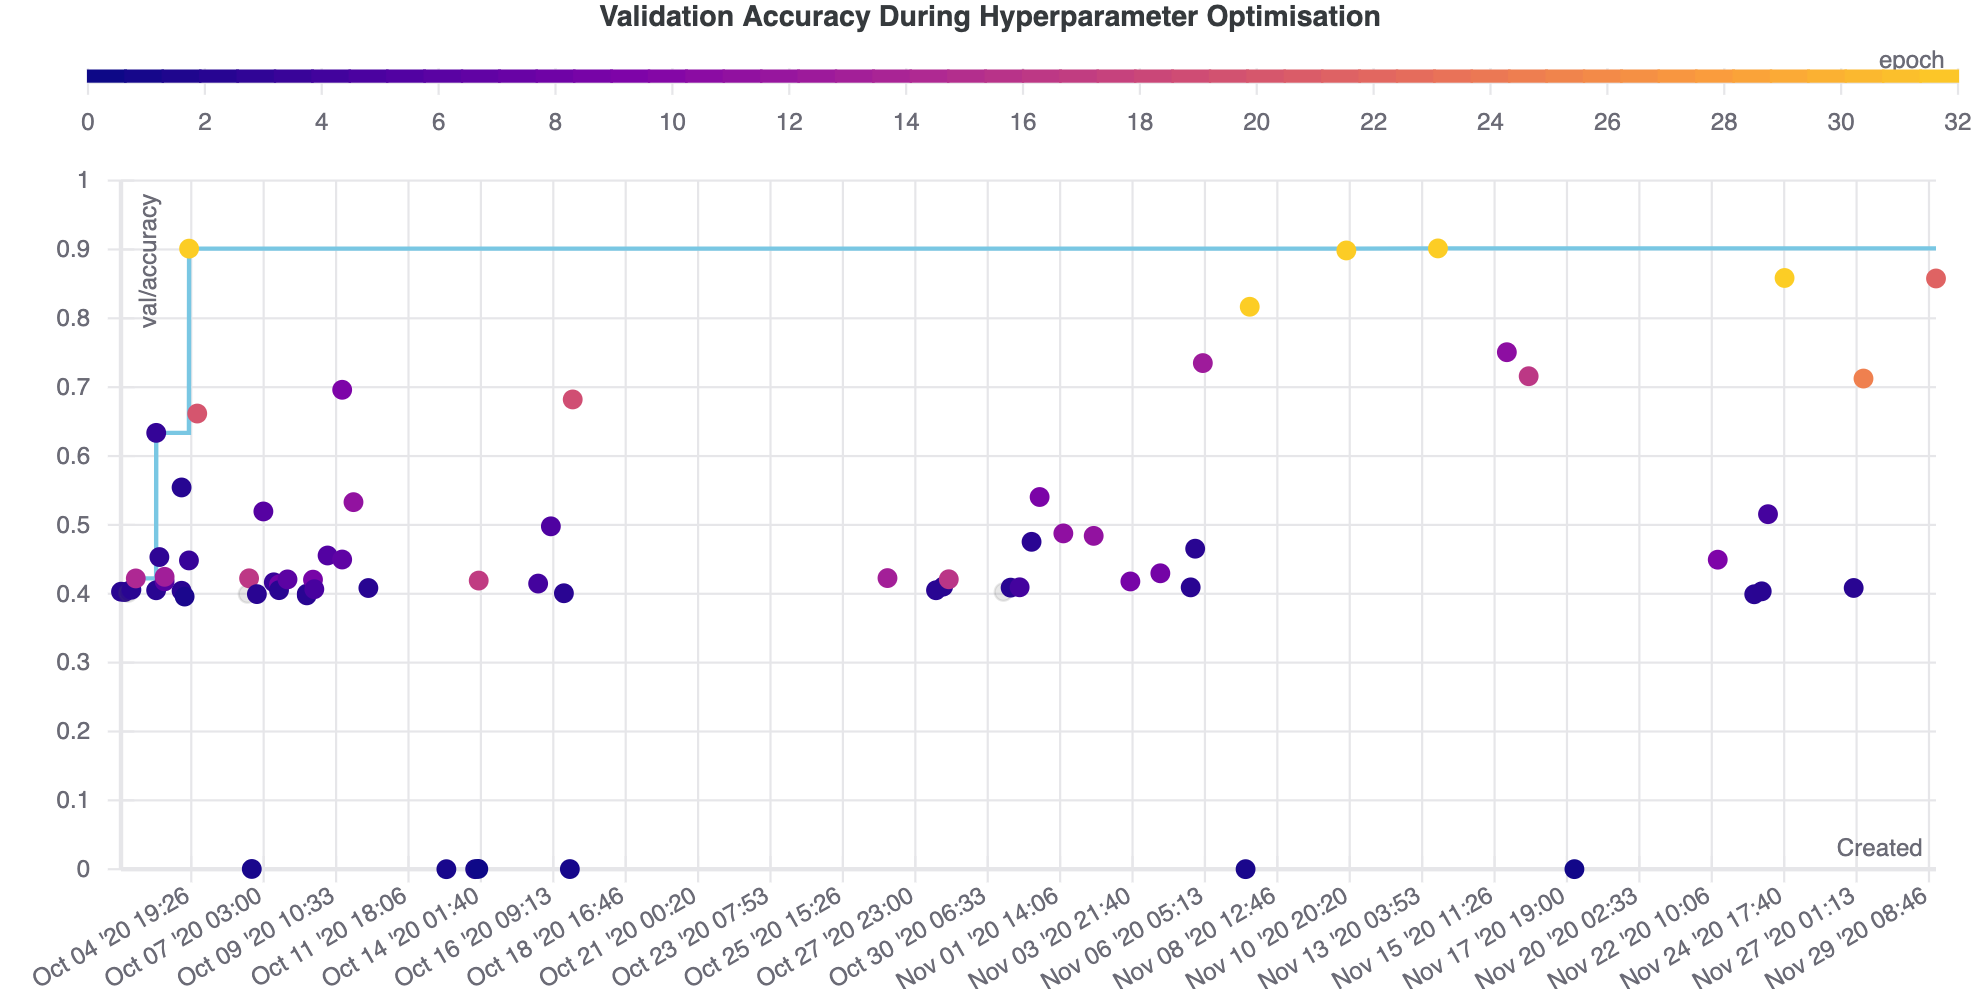
\includegraphics[width=\textwidth]{hyperparameter_optimisation_validation_accuracy.png}
        \label{fig:hyperparameter_optimisation_validation_accuracy}
        \caption{Validation accuracy throughout the hyperparameter optimisation process. Greyed out points correspond to models with a loss greater than 10.}
    \end{subfigure}
    \caption{A summary of validation loss and accuracy throughout the hyperparameter optimisation process. Each point represents a trained model, and its colour indicates how many epochs the model was trained for.}
    \label{fig:hyperparameter_optimisation_validation_loss_and_accuracy}
\end{figure}

\begin{figure}
    \centering
    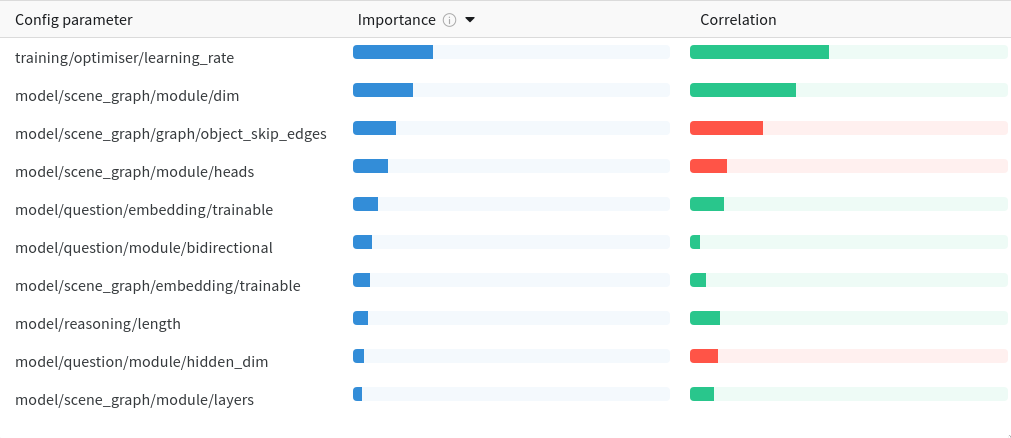
\includegraphics[width=\textwidth]{hyperparam_importance_and_correlation.png}
    \caption{Hyperparameter importance with respect to validation loss. Correlation is the linear correlation between each parameter and the validation loss, between -1 and 1. Parameter importance a value between 0 and 1, estimated by \textit{Weights \& Biases} \cite{wandb} by training a random forest classifier using configuration parameters as features and the validation loss as the target prediction.}
    \label{fig:hyperparam_importance_and_correlation}
\end{figure}

{\color{red} TODO: Correlation does not necessarily imply causation for parameter correlation to validation loss in \figureautorefname{ \ref{fig:hyperparam_importance_and_correlation}}}

\begin{figure}
    \centering
    \begin{subfigure}[l]{0.5\textwidth}
        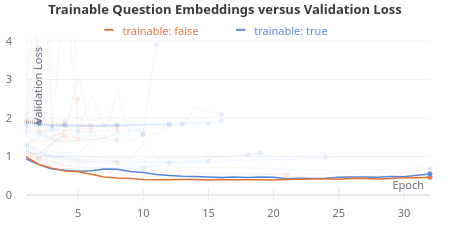
\includegraphics[width=\textwidth]{hyperparam_trainable_question_embedding_loss.png}
        \label{fig:hyperparam_trainable_question_embedding_loss}
        \caption{Validation Loss}
    \end{subfigure}
    \begin{subfigure}[r]{0.49\textwidth}
        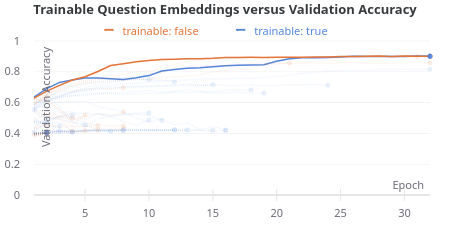
\includegraphics[width=\textwidth]{hyperparam_trainable_question_embedding_accuracy.png}
        \label{fig:hyperparam_trainable_question_embedding_accuracy}
        \caption{Validation Accuracy}
    \end{subfigure}
    \caption{}
    \label{fig:hyperparam_trainable_question_embedding_loss_and_accuracy}
\end{figure}
 
\begin{figure}
    \centering
    \begin{subfigure}[l]{0.5\textwidth}
        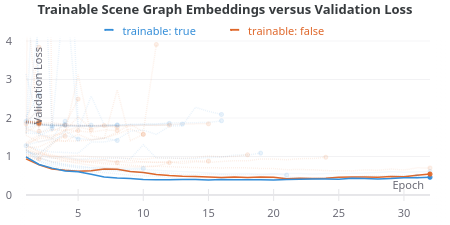
\includegraphics[width=\textwidth]{hyperparam_trainable_scene_embedding_loss.png}
        \label{fig:hyperparam_trainable_scene_embedding_loss}
        \caption{Validation Loss}
    \end{subfigure}
    \begin{subfigure}[r]{0.49\textwidth}
        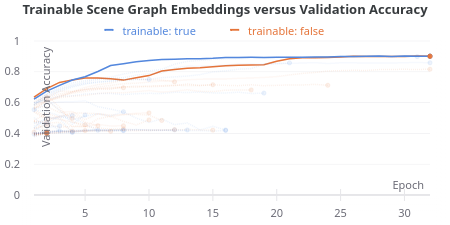
\includegraphics[width=\textwidth]{hyperparam_trainable_scene_embedding_accuracy.png}
        \label{fig:hyperparam_trainable_scene_embedding_accuracy}
        \caption{Validation Accuracy}
    \end{subfigure}
    \caption{}
    \label{fig:hyperparam_trainable_scene_embedding_loss_and_accuracy}
\end{figure}

\begin{figure}
    \centering
    \begin{subfigure}[l]{0.5\textwidth}
        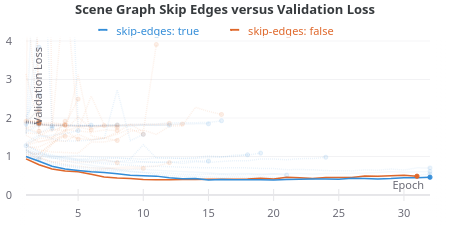
\includegraphics[width=\textwidth]{hyperparam_skip_edges_loss.png}
        \label{fig:hyperparam_skip_edges_loss}
        \caption{Validation Loss}
    \end{subfigure}
    \begin{subfigure}[r]{0.49\textwidth}
        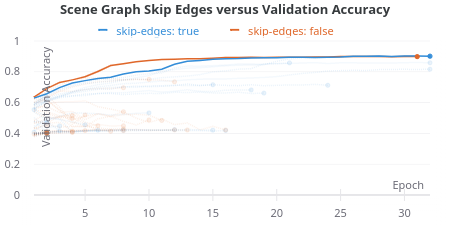
\includegraphics[width=\textwidth]{hyperparam_skip_edges_accuracy.png}
        \label{fig:hyperparam_skip_edges_accuracy}
        \caption{Validation Accuracy}
    \end{subfigure}
    \caption{}
    \label{fig:hyperparam_skip_edges_loss_and_accuracy}
\end{figure}
